\chapter{Fundamentação Teórica}

\section{Aprendizado de máquina}

Aprendizado de máquina, ou \textit{Machine Learning}, é uma área da
computação que emergiu de estudos relacionados ao reconhecimento de
padrões e inteligência artificial. Nesta área é contemplado o estudo e
implementação de algoritmos que conseguem aprender e fazer previsões
baseadas em dados. Esses algoritmos funcionam através da construção de
um modelo preditivo que tem como entrada um conjunto de treinamento
com dados de observações quaisquer. Desse modo as previsões são feitas
orientadas aos dados e não a partir de instruções estáticas de um
programa.

\section{Redes Neurais}

Diante das ferramentas disponíveis que tratam de aprendizado de
máquina, uma delas é a rede neural artificial.

Redes neurais artificiais são conjuntos de modelos inspirados por
redes neurais biológicas, usados para aproximar funções que dependem
de um número muito grande de entradas. De acordo com Mackay\cite{Mackay},
Redes neurais geralmente são especificadas utilizando 3 coisas:

\begin{itemize}

\item {\bf Arquitetura:} Especifica quais variáveis estão envolvidas
  na rede e quais as relações topológicas. Por exemplo, as variáveis
  envolvidas em uma rede neural podem ser os pesos das conexões entre
  os neurônios.

\item {\bf Regra de atividade:} A maioria dos modelos de rede neural
  tem uma dinâmica de atividade com escala de tempo curta. São regras
  locais que definem como as \textit{atividades} de neurônios mudam em
  resposta aos outros. Geralmente a regra de atividade depende dos
  parâmetros da rede.

\item {\bf Regra de aprendizado:} Especifica o modo com que os pesos
  da rede neural muda conforme o tempo. O aprendizado normalmente toma
  uma escala de tempo maior do que a escala referente a dinâmica de
  atividade. Normalmente a regra de aprendizado dependerá das
  \textit{atividades} dos neurônios. Também pode depender dos valores
  que são objetivos definidos pelo usuário e valores iniciais dos
  pesos.

\end{itemize}

Tomando imagens como exemplo, uma rede neural para reconhecimento de
texto pode ter como entrada o conjunto de pixels da imagem. Depois de
serem atribuídos os pesos para cada item da entrada, os próximos
neurônios serão ativados mediante a função de atividade
pré-definida. Os pesos são recalculados através da regra de
aprendizado e todo processo é repetido até uma condição determinada
pelo usuário.

\section{Convoluções}

Para entender redes neurais convolucionais, é necessário primeiro
entender o que são convoluções. Segundo Olah\cite{Olah}, uma
convolução pode ser vista como um somatório das probabilidades de
resposta de duas funções algébricas. Tendo como definição padrão de
convolução a seguinte expressão:

\begin{equation}
   (f*g)(c) = \sum\limits_{a}f(a)\cdot g(c-a)
\end{equation}

Onde {\bf \emph{f}} e {\bf \emph{g}} são duas funções, {\bf \emph{c}}
é o parâmetro de entrada para a função final e {\bf \emph{a}} é um
parâmetro de entrada escolhido para uma das funções, geralmente uma
diferença temporal.

Como podemos considerar que imagens são funções bidimensionais, é
comum realizar transformações por meio de convoluções. Estas
convoluções são executadas com uma função local pequena chamada de
``kernel''.

\begin{figure}[H]
\centering
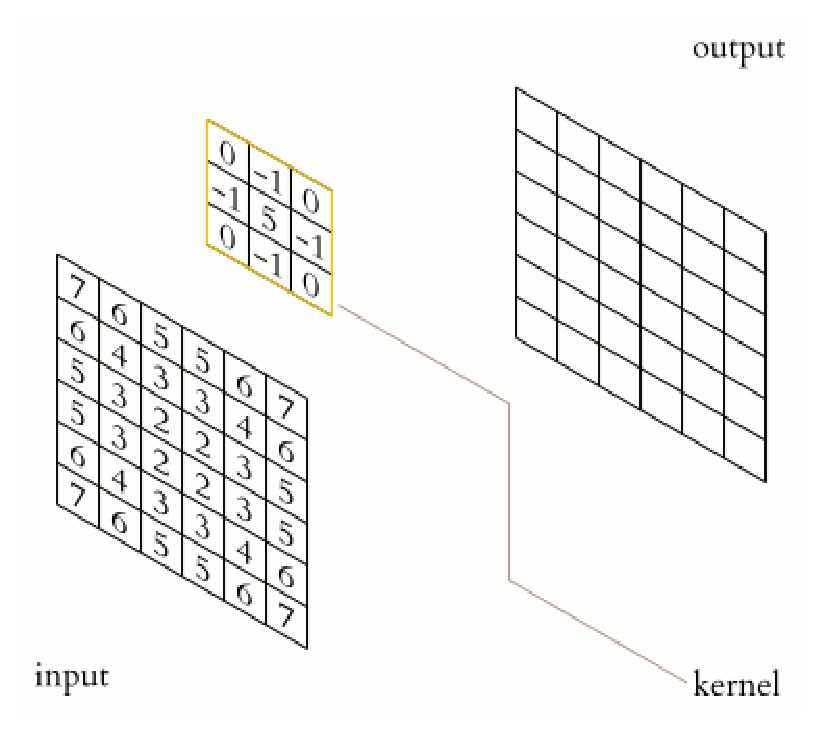
\includegraphics[scale=0.6]{imagens/fig1.eps}
\caption{Aplicação de uma função ``kernel'' sobre a função de uma
  imagem que é o ``input''.}
\label{fig:convolution_kernel}
\end{figure}

\subsection{Aplicação em redes neurais}

Redes neurais convolucionais são muito similares a redes neurais
comuns. De acordo com Karpathy\cite{Karpathy}:
\begin{quote}
  ``Arquiteturas de redes convolucionais assumem explicitamente que as
  entradas são imagens, o que nos permite cifrar algumas propriedades
  dentro da arquitetura. Essas então fazem a função de ativação mais
  eficiente de implementar e reduz drasticamente a quantidade de
  parâmetros na rede.'' (KARPATHY\cite{Karpathy}, 2015, tradução nossa).
\end{quote}

Portanto para o caso de reconhecimento de texto em imagens, as redes
neurais convolucionais fazem muito sentido.

\section{Aprendizado em profundidade}

O aprendizado em profundidade permite que modelos computacionais
compostos por múltiplas camadas de processamento possam aprender
representações de dados com múltiplos níveis de abstração\cite{LeCun}.

A solução de \textit{Deep learning} permite que computadores aprendam
a partir de experiencias e entendam o mundo em termos de uma
hierarquia de conceitos, com cada conceito definido em termos da sua
relação com conceitos mais simples. Juntando conhecimento de
experiência, essa abordagem evita a necessidade de ter operadores
humanos especificando formalmente todo o conhecimento que o computador
precisa. A hierarquia de conceitos permite que o computador aprenda
conceitos complexos construindo-os à partir de conceitos mais
simples. Desenhando um gráfico que mostra como esses conceitos são
construídos em cima de outros, o gráfico fica profundo, com muitas
camadas. Por esta razão, essa abordagem para IA é chamada de
Aprendizado em profundidade\cite{Goodfellow-et-al-2016-Book}.

\section{Redes neurais convolucionais de profundidade}

A grande vantagem na abordagem de redes neurais convolucionais de
profundidade (DCNN) para reconhecimento é que não é necessário um
extrator de características desenvolvido por um ser humano. Nas
soluções de \cite{Krizhevsky} e \cite{Goodfellow} é possível perceber
que foram usadas diversas camadas para o aprendizado das
características.

Em arquiteturas de profundidade, as funções de ativação dos neurônios
são unidades lineares retificadas (ReLU). Isso simplifica o uso de
\textit{backpropagation} e evita problemas de saturação, fazendo o
aprendizado ficar muito mais rápido.

\begin{figure}[H]
\centering
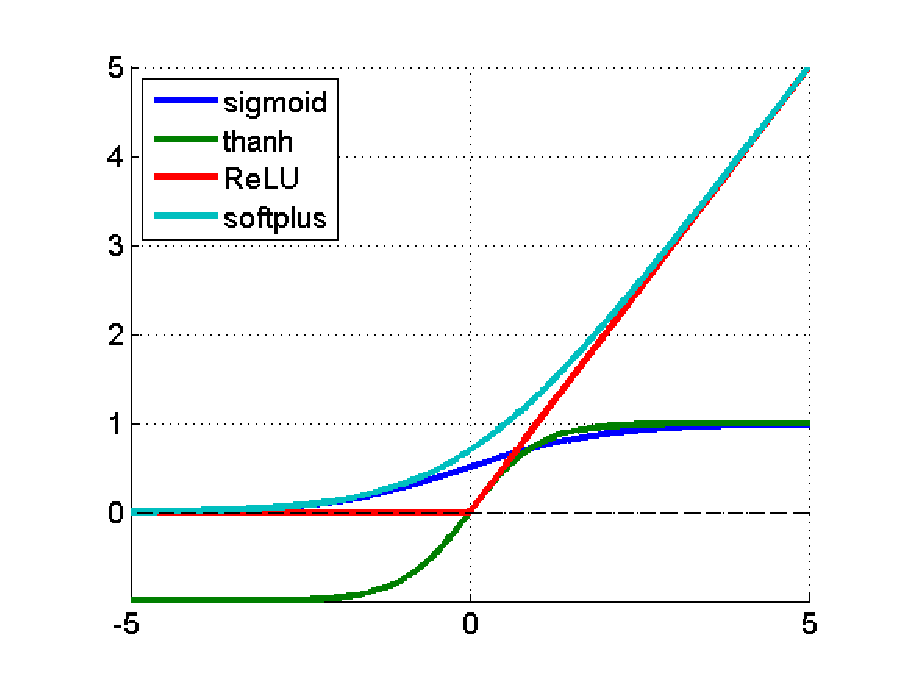
\includegraphics[scale=0.6]{imagens/activation_funcs.eps}
\caption{Comparação de funções de ativação.}
\label{fig:activation_funcs}
\end{figure}

Ao combinar o aprendizado em profundidade com redes convolucionais,
conseguimos tratar problemas muito mais complexos de classificação em
imagens. Assim problemas mais simples, como o reconhecimento de
textos, podem ser resolvidos cada vez mais rápido e facilmente.



Citar Jaderberg\cite{Jaderberg}
